% ****** Start of file apssamp.tex ******
%
%   This file is part of the APS files in the REVTeX 4.2 distribution.
%   Version 4.2a of REVTeX, December 2014
%
%   Copyright (c) 2014 The American Physical Society.
%
%   See the REVTeX 4 README file for restrictions and more information.
%
% TeX'ing this file requires that you have AMS-LaTeX 2.0 installed
% as well as the rest of the prerequisites for REVTeX 4.2
%
% See the REVTeX 4 README file
% It also requires running BibTeX. The commands are as follows:
%
%  1)  latex apssamp.tex
%  2)  bibtex apssamp
%  3)  latex apssamp.tex
%  4)  latex apssamp.tex
%
\documentclass[%
 reprint,
%superscriptaddress,
%groupedaddress,
%unsortedaddress,
%runinaddress,
%frontmatterverbose, 
%preprint,
%preprintnumbers,
%nofootinbib,
%nobibnotes,
%bibnotes,
 amsmath,amssymb,
 aps,
%pra,
%prb,
%rmp,
%prstab,
%prstper,
%floatfix,
]{revtex4-2}
\usepackage{kotex}
\usepackage{graphicx}% Include figure files
\usepackage{dcolumn}% Align table columns on decimal point
\usepackage{bm}% bold math
%\usepackage{hyperref}% add hypertext capabilities
%\usepackage[mathlines]{lineno}% Enable numbering of text and display math
%\linenumbers\relax % Commence numbering lines

%\usepackage[showframe,%Uncomment any one of the following lines to test 
%%scale=0.7, marginratio={1:1, 2:3}, ignoreall,% default settings
%%text={7in,10in},centering,
%%margin=1.5in,
%%total={6.5in,8.75in}, top=1.2in, left=0.9in, includefoot,
%%height=10in,a5paper,hmargin={3cm,0.8in},
%]{geometry}

\begin{document}


\title{약산의 분리와 적정 예비보고서}

\author{서울대학교 전기정보공학부 2018-12432 박정현}
 \email{alexist@snu.ac.kr}
\date{\today}% It is always \today, today,
             %  but any date may be explicitly specified

\begin{abstract}
아세트산, 살리실산이 혼합된 상태에서 $NaOH$으로 적정하여 약산, 강염기 적정을 이해한다. 이후에는 역상 크로마토그래피를 이용해 극성, 비극성 분자를 분리하고 해당 용액을 $NaOH$을 이용해 적정하여 농도를 측정하고 극성, 비극성, 소수성 상호작용에 대한 이해도를 높인다.
\end{abstract}

%\keywords{Suggested keywords}%Use showkeys class option if keyword
                              %display desired
\maketitle

%\tableofcontents

\section{\label{sec:level1}Introudction}
\section{\label{sec:level2}혼합 용액의 전체 산도}
아세트산 $CH_{3}(COOH)$, 그리고 살리실산($C_{6}H_{4}(OH)COOH$)은 모두 카복실기를 가지고 있어 약산에 해당한다. 아세트산은 $pK_{a}=4.75$ [2], 살리실산은 $pK_{a}=2.972$ [3]의 $pK_{a}$값을 가지고 있다. 이때 $NaOH(aq)$와의 반응은 아래와 같이 나타난다.

\begin{align}
	C_{7}H_{6}O_{3}(aq) \rightarrow C_{7}H_{5}O_{3}^{-}(aq) + H^{+}(aq) & pK_{a}=2.972\\
	C_{2}H_{4}O_{2}(aq) \rightarrow C_{2}H_{3}O_{2}^{-}(aq) + H^{+}(aq) & pK_{a}=4.75
\end{align}

이때 아래의 식이 성립한다.

\begin{align}
	1.07\times10^{-3} = \frac{[C_{7}H_{5}O_{3}^{-}][ H^{+}]}{[C_{7}H_{6}O_{3}]}\\
	1.76\times10^{-5} = \frac{[C_{2}H_{3}O_{2}^{-}][H^{+}]}{[C_{2}H_{4}O_{2}]}
\end{align}

초기 아세트산, 살리실산 농도를 각각 $[C_{2}H_{4}O_{2}]_{0}$, $[C_{7}H_{6}O_{3}]_{0}$라고 가정하고 $NaOH$용액을 이용해 적정한다고 가정하면 최종 당량점에서 아래의 식이 성립한다.

\begin{align}
	([C_{2}H_{4}O_{2}]_{0}+[C_{7}H_{6}O_{3}]_{0})V_{i} = [NaOH](V_{f}-V_{i})
\end{align}

살리실산의 $K_{a}$가 아세트산에 비해 100배 가량 크므로 2차당량점에서의 대부분 반응은 아세트산에 의한 것이다. 해당 반응식은 아래와 같다.

\begin{align}
	C_{2}H_{3}O_{2}^{-}(aq) + H_{2}O(l) \rightarrow C_{2}H_{4}O_{2}(aq)+ OH^{-}(aq)
\end{align}

이 때 $[C_{2}H_{3}O_{2}^{-}] \simeq [OH^{-}] = x$로 두면 아래의 식이 성립한다.

\begin{align}
	\frac{x^{2}}{[C_{2}H_{4}O_{2}]_{0}\frac{V_{i}}{V_{f}}-x} = \frac{10^{-14}}{1.76\times10^{-5}}
\end{align}

$NaOH$는 강염기이고 아세트산은 상대적으로 약산에 해당하므로 $x$가 충분히 작음을 알수있으므로 근사적으로 아래의 식이 성립한다.

\begin{align}
	[OH^{-}] \simeq 2.3\times10^{-5}\sqrt{[C_{2}H_{4}O_{2}]_{0}\frac{V_{i}}{V_{f}}}
\end{align}

만약 $[C_{2}H_{4}O_{2}]_{0} = 0M$이었을 경우 아래의 식이 성립할 것이다.

\begin{align}
	\frac{x^{2}}{[C_{2}H_{4}O_{2}]_{0}\frac{V_{i}}{V_{f}}-x} = \frac{10^{-14}}{1.07\times10^{-3}}
\end{align}
이러한 경우에도 마찬가지 방법으로 $pH$를 계산할 수 있으며 당량점에서의 $pH$는 약 $8$이상이므로 당량점 근처에서 색이 변화하게 된다.

따라서 $[C_{2}H_{4}O_{2}]_{0}\frac{V_{i}}{V_{f}}$가 $\sim 1mM$정도의 값을 가진다면 정량점은 $pH = 7.5\sim8.5$ 부근일 것이다. 페놀프탈레인의 변색번위가 $8.0~9.6$부근이므로 정량점 근처에서 색깔이 변화할 것을 알 수 있다.[3] 하지만 정량점보다 많은 양의 적정용액이 들어가야 변색이 되는데 이는 증류수에 $NaOH$을 바탕적정하여 해당값을 실험값에서 빼 정확한 당량점에서의 $NaOH$ 부피값을 측정할 수 있다.

\section{\label{sec:level2}산의 분리와 적정}
살리실산 각각의 분자 구조는 아래와 같다.[3] 아세트산의 경우 메틸기$CH_{3}$에 카복실기($COOH$)이 결합한 상태이므로 분자 구조에서 원자들 사이의 전기음성도 차이가 크고 비대칭적이므로 극성분자에 해당한다. 반면에 살리실산의 경우 대칭적인 육각구조에 카복실기와 $OH$가 결합한 상태이므로 아세트산과 비교했을 때 무극성 분자에 해당한다. 따라서 $C_{18}H_{37}$을 정지상, 극성이 높은 수용액을 이동상으로 사용하는 역상크로마토그래피에서 아세트산은 빠르게 흘러나오고, 살리실산은 크로마토그래피 상에서 느리게 이동하게 될것이다.

\begin{figure}[htbp]
	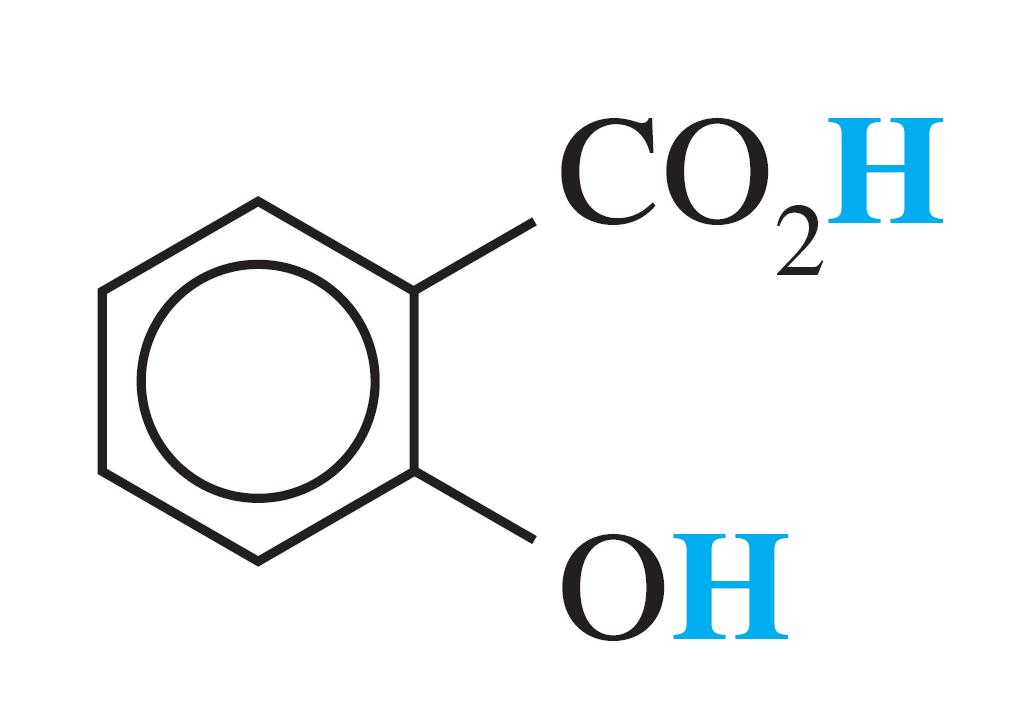
\includegraphics[width = 0.6\linewidth]{saly.png}% Here is how to import EPS art
	\caption{\label{fig:saly}살리실산 분자구조}
\end{figure}

\begin{align}
	A = \varepsilon b C
\end{align}

\section{\label{sec:level1}Experimental}
\section{\label{sec:level2}혼합 용액의 전체 산도}
피펫, $NaOH (2mM)$, 시험관, 뷰렛, 플라스크, 아세트산과 살리실산 혼합용액, 그리고 페놀프 탈레인 지시약을 준비한다. 피펫으로 아세트산, 살리실산 혼합용액 $1.0mL$를 비커에 담은 뒤 살살 저어주면서 $NaOH$용액으로 적정한다. 이후에는 $1.0mL$의 증류수를 $NaOH$용액으로 적정하여 바탕값을 측정한다.

\section{\label{sec:level2}산의 분리와 적정}
C18 카트리지, $10mL$와 $1mL$ 시린지, 플라스크, 아세트산과 살리실산 혼합용액을 준비한다. $5mL$ 정도의 증류수가 채워진 $10mL$의 시린지를 $C18$카트리지에 연결하여 밀어주며 카트리지를 세척한다. 이후에는 피펫을 이용해 $1.0mL$의 아세트산, 살리실산 혼합용액을 카트리지와 연결되어 있는 $10mL$ 시린지에 채운뒤 카트리지 상층부 위에 시료를 올린다. $1mL$ 시린지를 이용해 $1mL$씩 증류수로 카트리지를 용리해 나오는 용리액을 $1\sim 20$시험관에 받은뒤 각각을 $NaOH$용액으로 적정하여 산의 농도를 구한다.

\section{\label{sec:level1}Reference}
[1] 김희준, \textit{일반화학 실험}(자유아카데미, 2016)\\

[2] D.W. Oxtoby, H.P. Gillis, and L. Butler, \textit{Principles of Modern Chemistry} (Brooks/Cole, Australia, 2020). \\

[3] D.C. Harris, \textit{Quantitative Chemical Analysis} (W.H. Freeman and Co., New York, 2010). 


\end{document}
%
% ****** End of file apssamp.tex ******
